% Autor: Lukas Deeken
% Letzte Bearbeitung: 01.05.2022

\chapter{Elektrische Systeme} (zusammen mit Leon Löser)
Hier Geht mein dank an die Alumni aus dem Bereich der Elektrotechnik die diese ganze Reise mit ihrer fachlichen Refferenz und beispiellosen motivation erst möglich gemacht habe. Hervcorzuheben ist auch das schier endlose mas an gedult in anbetracht der Steilen lernkurve innerhalkb des teams. Besonders hervorzuheben sind hierbei Leon Löser, Eric Gorkow und Axel Lange. Danke euch.
\acfirst{IMD}
\section{Akkumulator}
Akkumulaotr layout und connecxtions
	AMS DCDC IMD TS Sensors AIR etc. mit visio

\subsection{AMS Master und Slave}
Layout welche funktionen sind wo, wozu gibt es funktionen etc.
Sprich Precharge auf AMS Master

\subsubsection{Precharge}


\subsubsection{AIR Detection}


\subsubsection{AMS}
Konkret BMS selber sprich LTC6811 etc

\subsubsection{HV Indicator}
Funktionsprinzip erklären Viper chip

\subsubsection{HV Messung}

\subsubsection{IMD Monitoring}

\subsubsection{Strommessung}
Isabellenhütte sensor

\subsection{HV DCDC}
Visio blockmodell
Erklärung ACFC
Berechnung excel etwas aufhübschen und anhängen
Teilberechnungen erklären

\section{HV Distribution}

\subsection{TSMP}
TSMP Wiederstände auslegung und steckverbidner plus kappen.

\subsection{BSPD}

VAC Sensorboard
Visio funktionsblockzeichnung
Implementierung der einzelnen funktionalen blöcke
schmitt trigger
integrator
Logik
\begin{figure}
	\centering
	\includegraphics[width=0.7\linewidth]{"bilder/BSPD Blockdiagramm"}
	\caption{}
	\label{fig:bspd-blockdiagramm}
\end{figure}

Die Aufgabe des BSPD ist es das Fahrzeug in dem Fall einer Störung des Gaspedales in einen Sicheren zustand zu überführen. Hierfür wird der Strom zu den Umrichtern als auch der Bremsdruck gemessen und beim eintreten eines im Regelwerk definierten schwellwertes für das gleichzeitige auftreten beider Signale muss das abschalten des Antriebes erfolgen. Das Folgende Blockdiagramm soll einen Überblick über den signalfluss ermöglichen.

Bei den Eingangsignalen handelt es sich um analoge spannungen. Für Sigfnalaufbereitung oder auch Digitalisierung der Signale werden Schitds Trigger einbgesetzt, Die Logik besteht aus diversen Logikgattern und die Set/reset Schaltung besteht aus Integrator Schaltungen m it nachgeschaltetetn schmidt triggern. Beim Shutdowncircuit handelt es sich um ein Solid State Relay welches von der BSPD Logik schlussendlich angestuert werden soll, ein öffnen des Shutdwon circuit führt damnit zu einem Herunterfahren des Antriebes.

Zur Auslegung von Schmidt Triggern
\begin{figure}
	\centering
	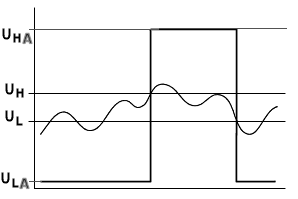
\includegraphics[width=0.5\linewidth]{bilder/Schmitt-trigger-diagramm.png}
	\caption{}
	\label{fig:schmitt-trigger-diagramm}
\end{figure}

Die Funktionsweise eines Schmitt Trigger kann anhand des Bildes erkannt werden. Er ermöglicht es ein analoges Signal in ein Digitales umzuwandeln, dabei ist es möglich festzulegen welche Spannungspegel am Ausgang des Schmitt Trigger anliegen (\glsc{symb:U_HA} und \glsc{symb:U_LA}) und bei welchen Spannungspegeln der Trigger High respektive Low schalten soll (\glsc{symb:U_H}und \glsc{symb:U_L}). Das vorliegen unterschiedilcher Pegel zum Schalten wird Hysterese genannt. Grund für das vorliegen ist das verhindern des rapiden Umschaltens zwischen High und Low direkt an dem Schwellwert aufgrund von Signalrauschen.

\begin{figure}
	\centering
	\includegraphics[width=0.7\linewidth]{"bilder/TPS Failure detection"}
	\caption{}
	\label{fig:tps-failure-detection}
\end{figure}

\begin{figure}
	\centering
	\includegraphics[width=0.7\linewidth]{"bilder/nichtinvertierender Trigger"}
	\caption{}
	\label{fig:nichtinvertierender-trigger}
\end{figure}

Folgend Beispielhaft die Auslegung eines Nicht Invertierenden Schmitt Triggers wie er im Bild unten zu sehen ist. Die andere Ausführung ist die eines Invertierenden.

Zur Berechnung sollten sich \glsc{symb:U_HA} und \glsc{symb:U_LA} sowie \glsc{symb:U_H} und \glsc{symb:U_L} aus dem Betriebsfall ergeben. R\textsubscript{1} sowie R\textsubscript{3} können frei gewählt werden. R\textsubscript{1} ist hierbei der Verbund aus R\textsubscript{3} und R\textsubscript{4}.

Die beiden folgenden Gleichung liegen zu Grunde

\begin{equation}
	\label{eqn:Obere Hysteresespannung Schmitt Trigger}
	\glsc{symb:U_H} = \glsc{symb:U_ref} + (\glsc{symb:U_HA} - \glsc{symb:U_ref}) * \dfrac{R\textsubscript{1}} {R\textsubscript{1}+R\textsubscript{2}}
	mit R\textsubscript{1}=\dfrac{R\textsubscript{3}*R\textsubscript{4}}{R\textsubscript{3}+R\textsubscript{4}}
\end{equation}

Und

\begin{equation}
	\label{eqn:Untere Hysteresespannung Schmitt Trigger}
	\glsc{symb:U_L}=\glsc{symb:U_ref}-(\glsc{symb:U_ref}-\glsc{symb:U_HA})*\dfrac{R\textsubscript{1}}{R\textsubscript{1}+R\textsubscript{2}}
\end{equation}

Mit den folgenden Gleichungen lassen sich R\textsubscript{2} und R\textsubscript{4} bestimmen

\begin{equation}
	\label{eqn:Berechnung R2 Schmitt Trigger}
	R\textsubscript{2} = R\textsubscript{1} * \dfrac{\glsc{symb:U_HA} - \glsc{symb:U_LA}} {\glsc{symb:U_H} - \glsc{symb:U_L}}
\end{equation}

\begin{equation}
	\label{eqn:Berechnung Uref Schmitt Trigger}
	\glsc{symb:U_ref} = (\glsc{symb:U_H} - \glsc{symb:U_LA}) * \dfrac{R\textsubscript{2}} {R\textsubscript{1} + R\textsubscript{2}} + \glsc{symb:U_LA}
\end{equation}

\begin{equation}
	\label{eqn:Berechnung R4 Schmitt Trigger}
	R\textsubscript{4} = R\textsubscript{3} * \dfrac{\glsc{symb:VCC}-\glsc{symb:U_ref}} {\glsc{symb:U_ref}}
\end{equation}

Zur Auslegung von Integratoren

Übersicht über die BSPD Logik


\subsection{Discharge}
PTC berechnung

\section{TSAL}

\subsection{Logik auf Discharge}

\subsection{Logik auf AMS Master}